\documentclass{../main.tex}{}

\begin{document}
Reinforcement learning (RL) is an optimization framework. A problem can be considered a reinforcement learning problem if it can be framed in the following way: Given an enviroment in which an agent can take actions, receiving a reward for each action, find a policy that maximizes the expected cumulative reward that the agent will obtain by acting in the environment.

\begin{figure}[h]
    \centering
    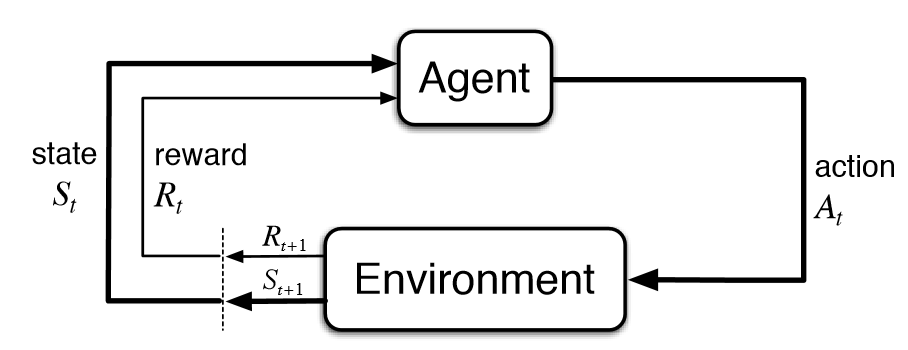
\includegraphics[width=0.8\textwidth]{images/rl-loop}
    \caption{Reinforcement learning loop}
    \label{fig:rl-loop}
\end{figure}

\end{document}
